\documentclass[
mode=present,
paper=smartboard,
size=20pt,
]{powerdot}
\usepackage{latabbr}
\usepackage{verbatim}
\usepackage[utf8]{inputenc}

%% Spacing macros (with default argument).
\newcommand\vsp{\vspace{-16mm}}
\makeatletter\renewcommand{\verbatim@font}{\footnotesize\tt}\makeatother
\newcommand{\clopt}[1]{\texttt{{-}#1}}

\title{GnuPG for Beginners}
%\subtitle{The GNU Privacy Guard}
\author{%
  Tristan Miller\\
  Ubiquitous Knowledge Processing Lab\\
  Department of Computer Science\\
  Technische Universit\"at Darmstadt
}
\date{August 16, 2016}
\pdsetup{
  lf={GnuPG for Beginners},
  palette={blue},
}

\begin{document}
\maketitle

\begin{slide}[toc=]{Overview}
  \begin{itemize}
  \item Introduction of symmetric and public-key cryptography
  \item GnuPG: A free implementation of the OpenPGP standard
    \begin{itemize}
    \item Creating and managing keys
    \item Encrypting and decrypting documents
    \item Generating and verifying digital signatures
    \item GnuPG trust model
    \item Front ends
    \end{itemize}
  \end{itemize}
\end{slide}

%=============================================================================
\section{Background}
%=============================================================================
\begin{slide}{Symmetric ciphers}
  \begin{itemize}
  \item A \textbf{symmetric cipher} uses the same key for encryption
    and decryption.
  \item Two parties communicating using a symmetric cipher must agree
    on the key beforehand.
  \item The sender encrypts a message using the key,
    sends it to the receiver, and the receiver decrypts the message
    using the key.
  \item Examples: ROT13, AES, 3DES, Blowfish.
  \item Advantage: hard to crack, provided the key is big enough
    (128~bits is standard).
  \item Disadvantage: How to securely communicate the key?
  \end{itemize}
\end{slide}

\begin{slide}[toc=]{Symmetric ciphers}
\centering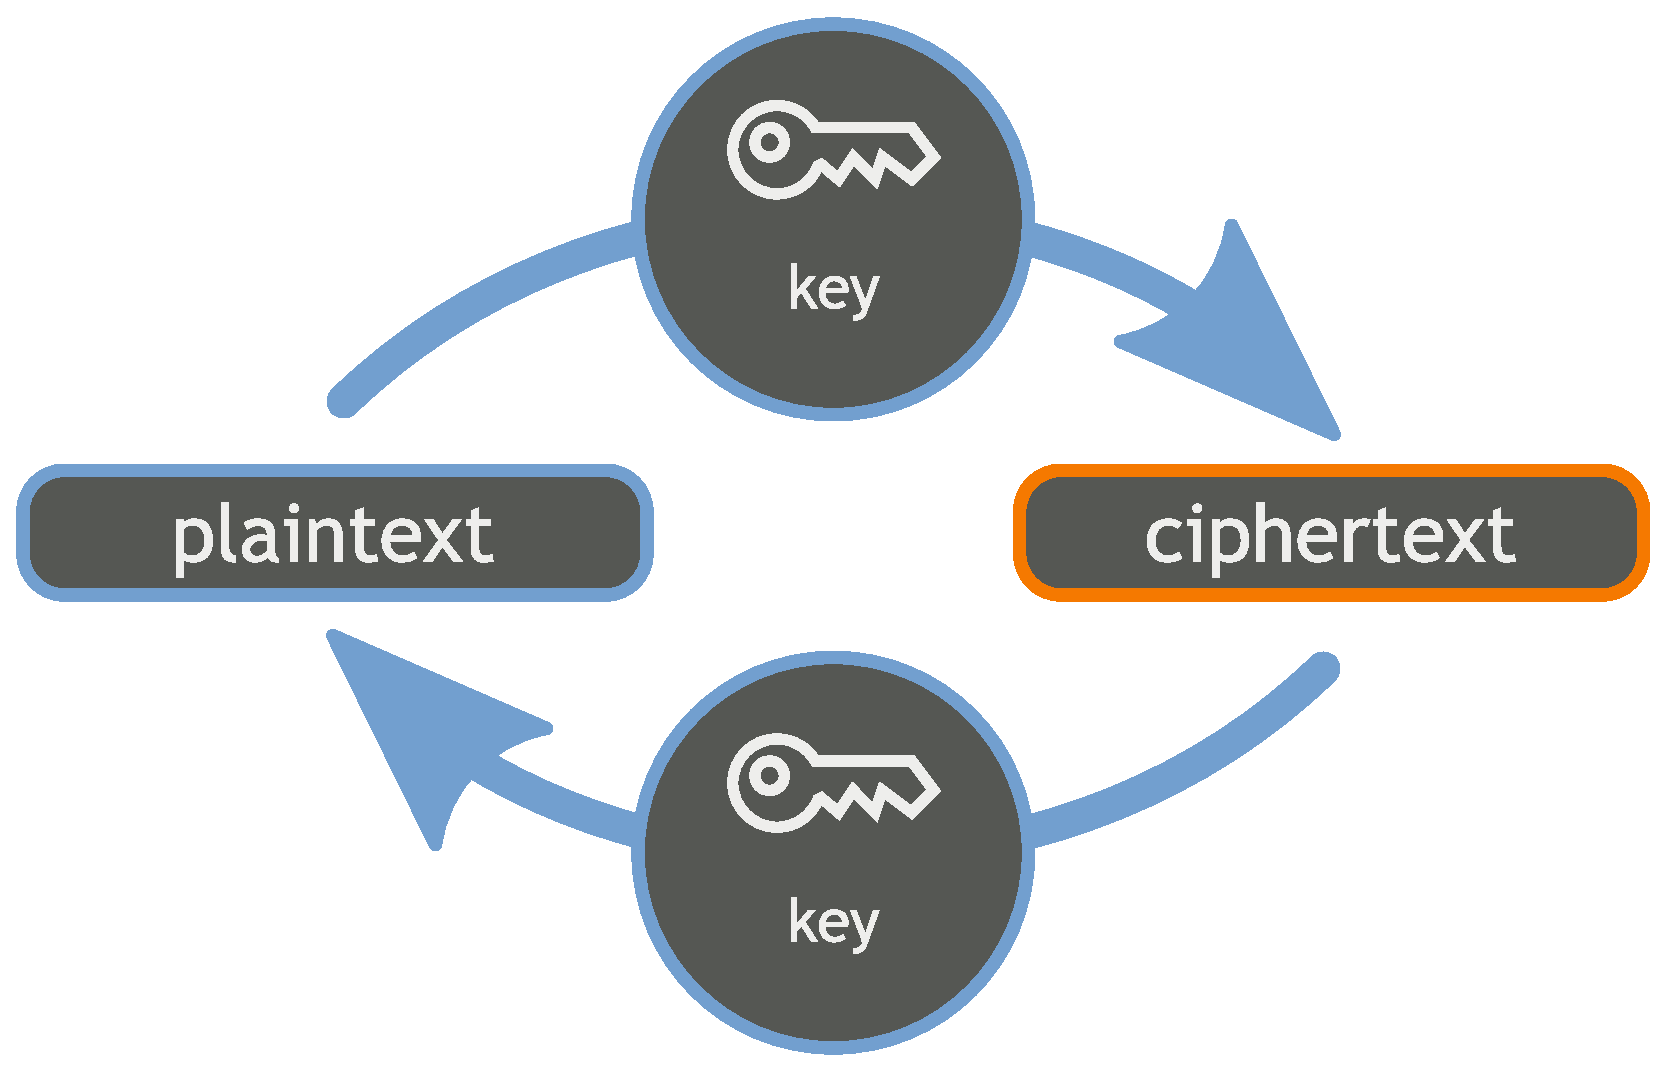
\includegraphics[width=0.9\linewidth]{images/Orange_blue_symmetric_cryptography_en}
\end{slide}

\begin{slide}{Public-key ciphers}
  \begin{itemize}
  \item \textbf{Public-key} ciphers use a pair of keys:
    \begin{itemize}
    \item The \textbf{public key} is given to anyone who wishes to
      communicate and is used to encrypt a message.
    \item The \textbf{private key} is kept secret and is used to
      decrypt a message.
    \end{itemize}
  \item Advantage: simplified key exchange.
  \item Disadvantage: easier to crack, so key sizes must be much
    larger ($\geq$2048~bits is standard).
  \item \textbf{Hybrid ciphers} combine elements of both symmetric and
    public-key encryption.
  \end{itemize}
\end{slide}

\begin{slide}[toc=]{Public-key ciphers}
\centering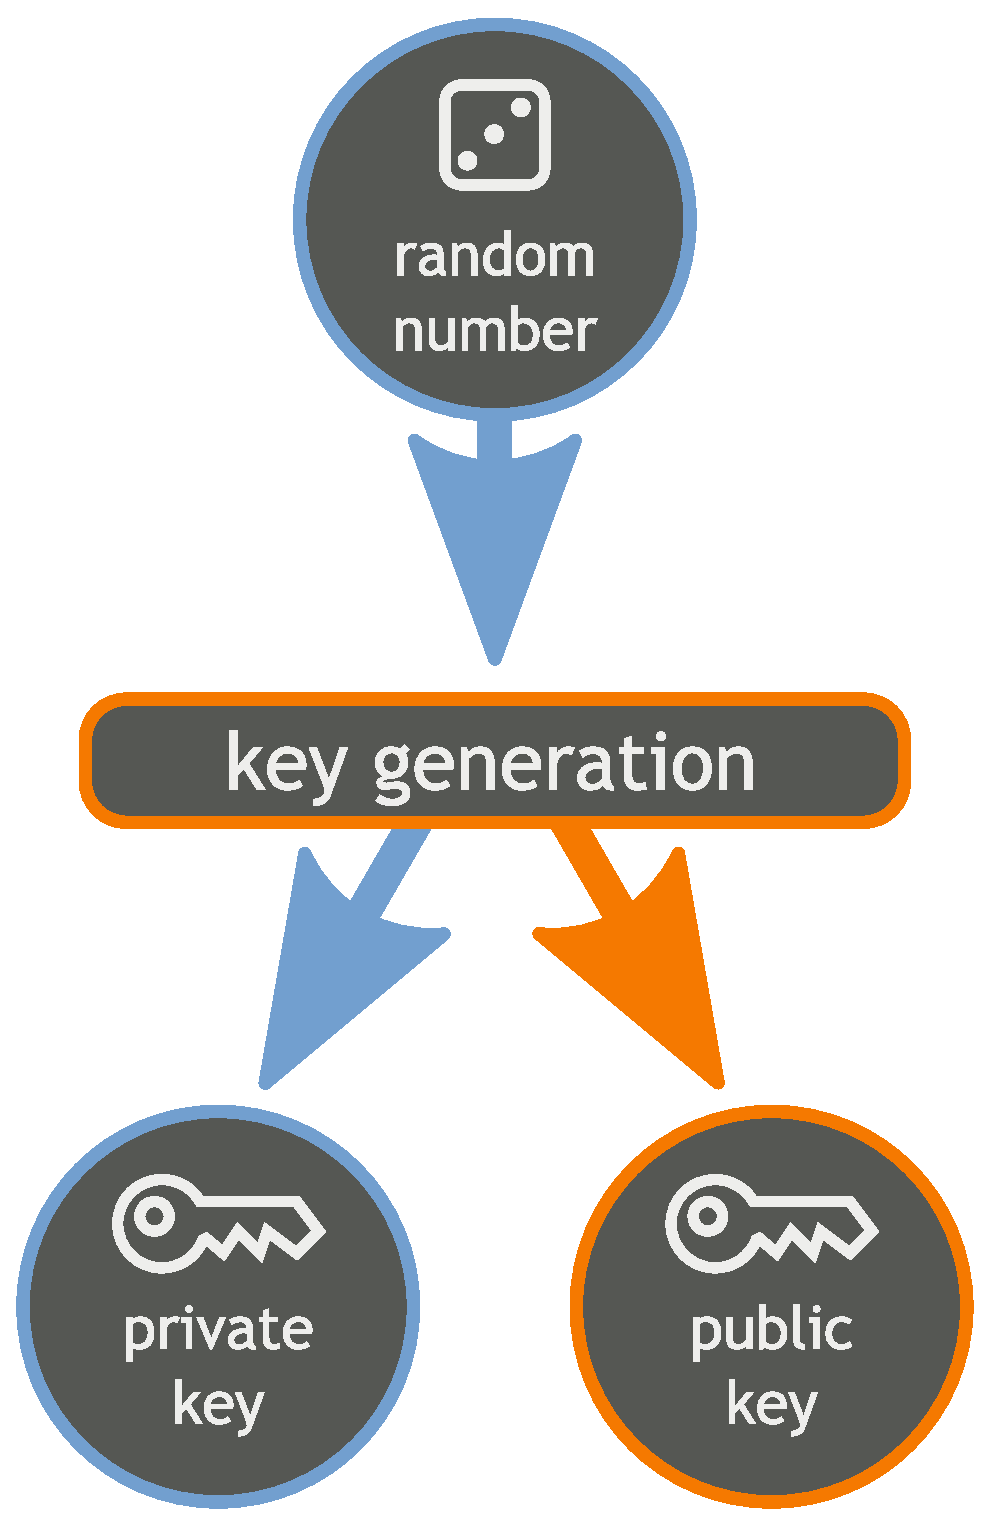
\includegraphics[width=0.35\linewidth]{images/Orange_blue_public_private_keygeneration_en.eps}
\end{slide}

\begin{slide}[toc=]{Public-key ciphers}
\centering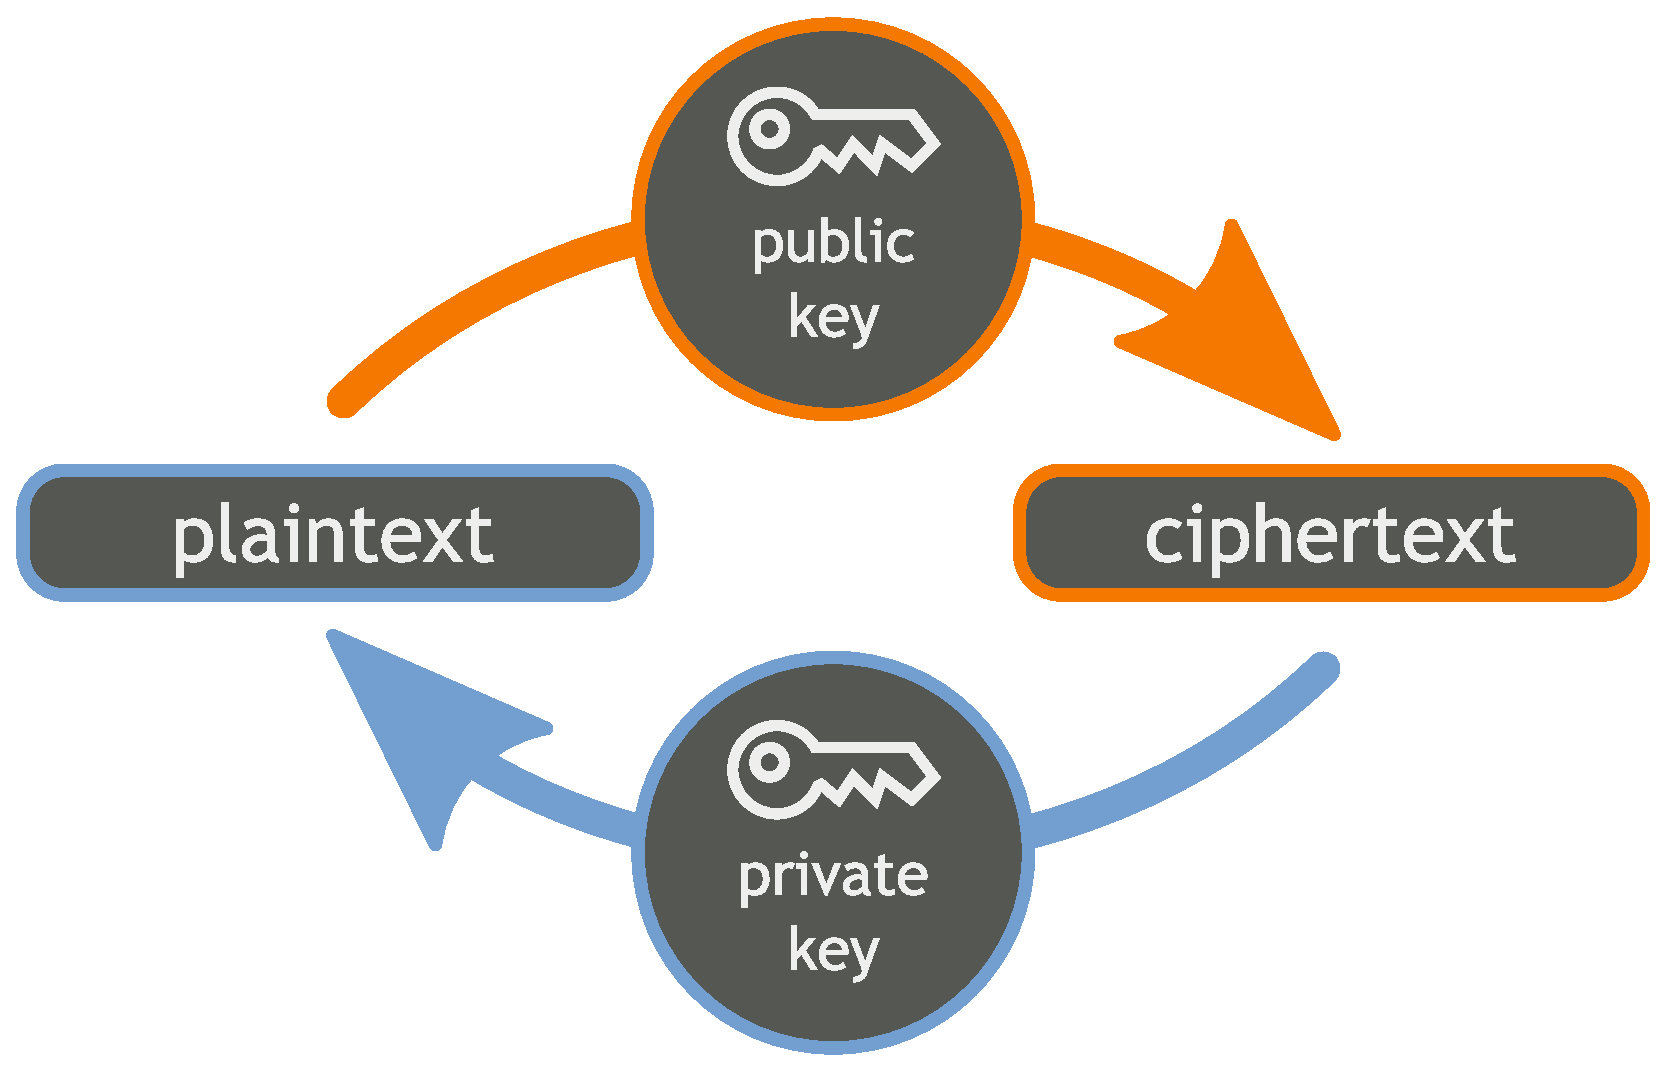
\includegraphics[width=0.9\linewidth]{images/Orange_blue_public_key_cryptography_en.eps}
\end{slide}

\begin{slide}{Digital signatures}
  \begin{itemize}
  \item A document's \textbf{digital signature} is the result of
    applying a one-way hash function to the document.
  \item The hash is then encrypted using the signer's \textbf{private
      key}.
  \item To verify the signature, the recipient decrypts the hash using
    the signer's \textbf{public key}.
  \item If the decrypted hash value matches the actual hash value of
    the document (as calculated by the recipient), then the recipient
    can be sure that the document he has received was exactly the same
    one the signer sent.
  \end{itemize}
\end{slide}

\begin{slide}[toc=]{Digital signatures}
\centering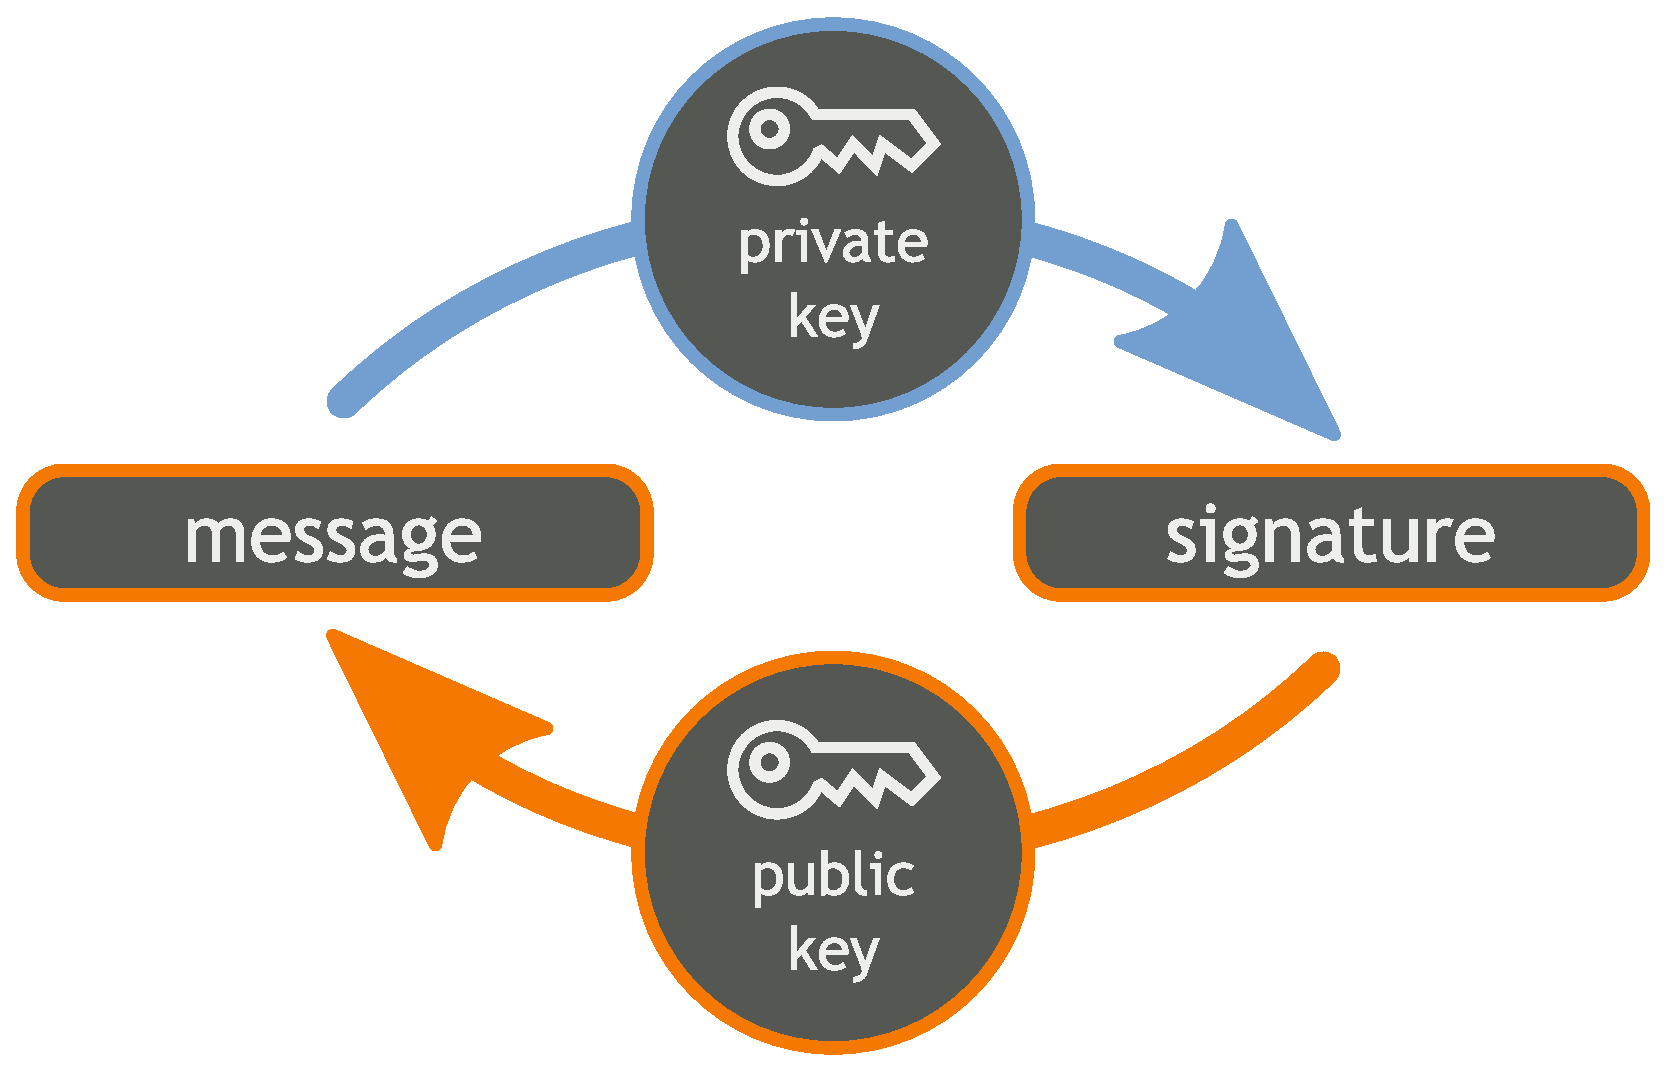
\includegraphics[width=0.9\linewidth]{images/Orange_blue_digital_signature_en.eps}
\end{slide}

\begin{slide}{Web of trust}
  \begin{itemize}
  \item When you have faith that a certain public key belongs to a
    certain person, you can add your digital signature to that public
    key and then republish it.
  \item However, it would be awkward for you to have to personally
    verify and sign every single public key you encounter.
  \item OpenPGP addresses this problem with a mechanism
    known as the \textbf{web of trust}.
  \item In the web of trust model, responsibility for validating
    public keys is delegated to people you trust.
  \end{itemize}
\end{slide}

\begin{slide}[toc=]{Web of trust}
\centering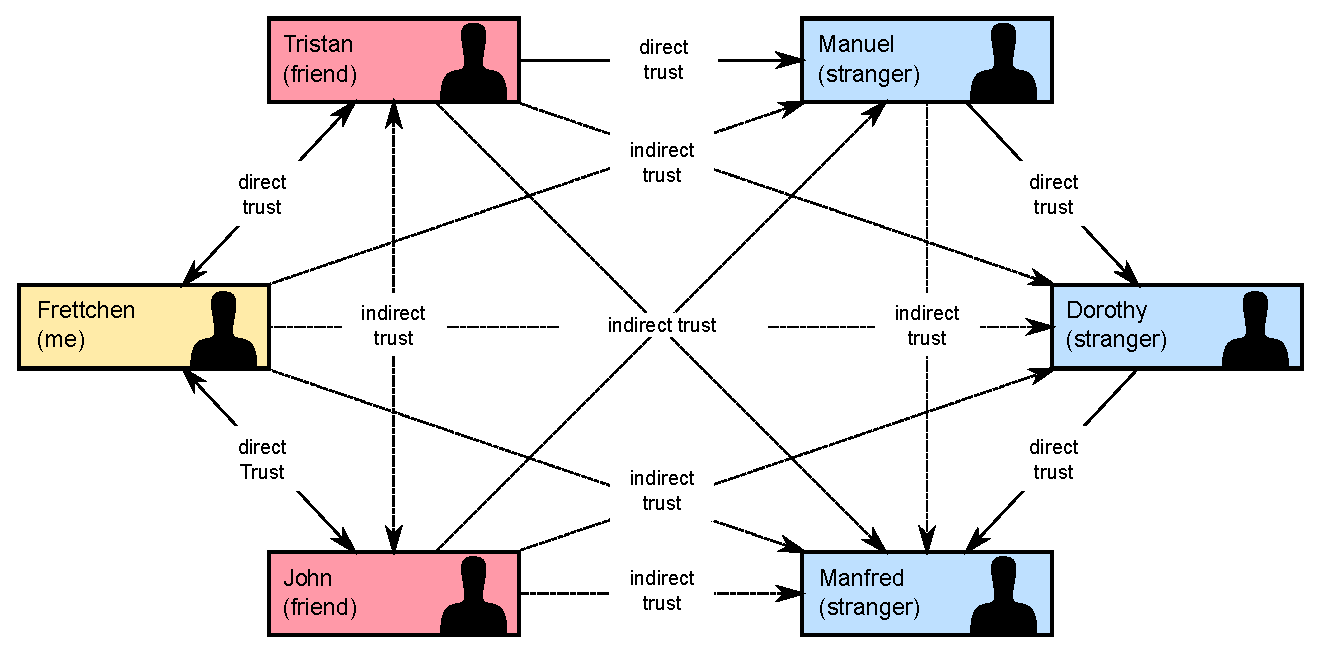
\includegraphics[width=\linewidth]{images/Web_of_Trust.eps}
\end{slide}


%=============================================================================
\section{Why use GnuPG?}
%=============================================================================
\begin{slide}{Software distribution}
  If you distribute software on the Internet, there are many reasons
  to digitally sign your packages:\\[1ex]
  \begin{itemize}
  \item packages cannot be tampered with without breaking the signature
  \item corrupted downloads will break the signature
  \item encapsulated signatures are supported and encouraged by major packaging formats: JAR (Maven), RPM, deb, \etc
  \end{itemize}
\end{slide}

\begin{slide}{Authenticating e-mail}
  \begin{itemize}
  \item By making it a policy of yours to always sign important
    e-mails, you can prevent e-mails from being forged in your name.
  \item When your colleagues sign their e-mails,
    you can always be sure you know who you're communicating with.
  \item Signing e-mails prevents deniability---if you receive a signed
    document from someone, they cannot later claim that they did not
    produce it.
  \end{itemize}
\end{slide}

\begin{slide}{Encrypting e-mail}
  Encrypting e-mails containing proposals, results, and publication
  drafts reduces the following risks:\\[1ex]
  \begin{itemize}
  \item sensitive communications intercepted by or leaked to press
  \item research results copied and published by unscrupulous
    colleagues or students
  \item corporate espionage on important projects with business
    research partners
  \item private documents accidentally sent to wrong e-mail address
  \end{itemize}
\end{slide}

\begin{slide}{Protecting personal data}
  GnuPG's symmetric-key encryption can be used to protect sensitive
  documents stored on your own (or remote) computers.  For instance:\\[1ex]
  \begin{itemize}
  \item experiment results
  \item personal data on experiment volunteers
  \item password lists
  \item bank and credit card statements
  \end{itemize}
\end{slide}


%=============================================================================
\section{Acquiring the software}
%=============================================================================

\begin{slide}{GnuPG \vs PGP \vs OpenPGP}
  \begin{itemize}
  \item \textbf{PGP}: first developed and freely released by Phil Zimmerman
  \item PGP later commercialized; now a proprietary system
  \item encryption method standardized as \textbf{OpenPGP}
  \item \textbf{GnuPG} is GNU's free implementation of the OpenPGP standard
  \item other implementations of OpenPGP exist, but GnuPG is free and
    popular
  \end{itemize}
\end{slide}

\begin{slide}{Installing GnuPG}
  \begin{itemize}
  \item Download from \url{https://gnupg.org/} or from your OS's package manager.
  \item Compile from source or fetch a binary package for a supported
    system:
    \begin{itemize}
    \item GNU/Linux
    \item Mac OS X
    \item Android
    \item Microsoft Windows
    \end{itemize}
  \item Third-party GUIs are available, but an understanding of the underlying
    command-line version is helpful.
  \end{itemize}
\end{slide}

%=============================================================================
\section{Managing keys}
%=============================================================================

\begin{slide}[method=direct]{Generating keypairs}
  \begin{itemize}
  \item All GnuPG functions are invoked through the \texttt{gpg} command.
  \item The command-line option \clopt{-gen-key} is used to create a new
  primary keypair.
  \end{itemize}
\begin{verbatim}
$ gpg --gen-key
gpg (GnuPG) 2.0.24; Copyright (C) 2013 Free Software Foundation, Inc.
This is free software: you are free to change and redistribute it.
There is NO WARRANTY, to the extent permitted by law.

Please select what kind of key you want:
   (1) RSA and RSA (default)
   (2) DSA and Elgamal
   (3) DSA (sign only)
   (4) RSA (sign only)
Your selection?
\end{verbatim}
\end{slide}

\begin{slide}[method=direct,toc=]{Generating a new keypair}
  \begin{itemize}
  \item You will be prompted for a key type and key size.
  \item The defaults (2048-bit RSA keys, in recent GnuPG versions) are
    generally sensible.
  \item Larger key sizes provide extra security at the cost of speed;
    if future-proofing is important for you, use the maximum key size
    of 4096 bits.
  \end{itemize}
\begin{verbatim}
Your selection? 1
RSA keys may be between 1024 and 4096 bits long.
What keysize do you want? (2048)
\end{verbatim}
\end{slide}

\begin{slide}[method=direct,toc=]{Generating a new keypair}
  \begin{itemize}
  \item Next, you must choose an expiration date.
  \item For most users, a key that does not expire is adequate.
  \item Some people prefer to set an expiry date (say, two years) as a
    safeguard. You can periodically extend the expiry date if your key
    is still in use.
  \end{itemize}
\begin{verbatim}
Please specify how long the key should be valid.
         0 = key does not expire
      <n>  = key expires in n days
      <n>w = key expires in n weeks
      <n>m = key expires in n months
      <n>y = key expires in n years
Key is valid for? (0)
\end{verbatim}
\end{slide}

\begin{slide}[method=direct,toc=]{Generating a new keypair}
  \begin{itemize}
  \item You must now provide a user ID.
  \item It is possible to add additional user IDs later in case you
    want to use the key in two or more contexts.
  \item A user ID should be created carefully since it cannot be
    edited after it is created!
  \item Avoid using the ``Comment'' field without good reason.
  \end{itemize}
\vsp
\begin{verbatim}
GnuPG needs to construct a user ID to identify your key.

Real name: Frettchen Rättchen
Email address: frettchen@dfki.de
Comment: 
You are using the `utf-8' character set.
You selected this USER-ID:
    "Frettchen Rättchen <frettchen@dfki.de>"

Change (N)ame, (C)omment, (E)mail or (O)kay/(Q)uit?
\end{verbatim}
\end{slide}

\begin{slide}[method=direct,toc=]{Generating a new keypair}
  \begin{itemize}
  \item Finally, you must enter a \textbf{passphrase} to protect your
    private key.
  \end{itemize}
\vsp
\begin{verbatim}
You need a Passphrase to protect your secret key.    

Enter passphrase: 
\end{verbatim}

  \begin{itemize}
  \item Because this passphrase protects access to your PGP identity, it
    should be carefully chosen.  It must be long enough to be secure,
    but also easy for you to remember and type.
  \item At \url{http://www.diceware.com/} you will find a method of
    generating long but easy-to-remember passphrases by combining five
    English or German words.

    Example: \texttt{distel ist landen kammer puffen}
  \end{itemize}
\end{slide}

%\makeatletter\renewcommand{\verbatim@font}{\tiny\tt}\makeatother
\begin{slide}[method=direct]{Your public keyring}
  \begin{itemize}
  \item Your \textbf{keyring} is a list of all public keys you have
    generated or imported.  You can view it with the
    \clopt{-list-keys} option:
  \end{itemize}
\begin{verbatim}
$ gpg --list-keys
/home/frettchen/.gnupg/pubring.gpg
----------------------------------
pub   2048R/4116CBB0 2016-08-15
uid       [ultimate] Frettchen Rättchen <frettchen@dfki.de>
sub   2048R/FA659AB0 2016-08-15

pub  1024D/EFBF4915 2003-10-24 Tristan Miller (Research scientist) <tristan.miller@dfki.de>
uid                            Tristan Miller <psychonaut@nothingisreal.com>
sub  1024g/B40BE860 2003-10-24
\end{verbatim}
\end{slide}

\begin{slide}[method=direct,toc=]{Your public keyring}
  \begin{itemize}
  \item Most command-line arguments dealing with keys let you specify
    a particular key or set of keys.  You can use the key's ID or any
    part of the user ID.  For example:
  \end{itemize}
\begin{verbatim}
$ gpg --list-keys Tristan
pub  1024D/EFBF4915 2003-10-24 Tristan Miller (Research scientist) <tristan.miller@dfki.de>
uid                            Tristan Miller <psychonaut@nothingisreal.com>
sub  1024g/B40BE860 2003-10-24
\end{verbatim}
\end{slide}

%\makeatletter\renewcommand{\verbatim@font}{\tiny\tt}\makeatother
\begin{slide}[method=direct]{Revocation certificates}
  \begin{itemize}
  \item If you forget your passphrase or if your private key is
    compromised or lost, a \textbf{revocation certificate} may be
    published to notify others that the public key should no longer be
    used.
  \end{itemize}
\vsp
\begin{verbatim}
$ gpg --output revoke.asc --gen-revoke Frettchen

sec  2048R/4116CBB0 2016-08-15 Frettchen Rättchen <frettchen@dfki.de>

Create a revocation certificate for this key? (y/N) y
Please select the reason for the revocation:
  0 = No reason specified
  1 = Key has been compromised
  2 = Key is superseded
  3 = Key is no longer used
  Q = Cancel
(Probably you want to select 1 here)
Your decision? 
\end{verbatim}
  % \begin{itemize}
  % \item The revocation certificate should be printed out and stored in
  %   a safe place.
  % \end{itemize}
\end{slide}

%\makeatletter\renewcommand{\verbatim@font}{\scriptsize\tt}\makeatother
\begin{slide}[method=direct]{Exporting a public key}
  \begin{itemize}
  \item To communicate with others you must exchange public keys.
  \item To export a public key on your keyring, use the
    \clopt{-export} option.
  \item By default, keys are exported as binary data, but you can
    specify an ASCII encoding using the \clopt{-armor} option.
  \end{itemize}
\vsp
\begin{verbatim}
$ gpg --armor --export Frettchen
-----BEGIN PGP PUBLIC KEY BLOCK-----
Version: GnuPG v2

mQENBFex0P4BCADR8+CMx/j8mIMQEMWjS/2GOSth1tR5mSwuk31oPMn0xtPTY+oK
BshOMDJjujJew/+aJBu2rTBGQdfza4W/jBLy/uwU8C92+Rp6SBsPw9P+f0g297pm
                             ...
WWKwsmkDsqlJzdDVsFHYYJTHy+MUBRzrVbuG8lscCeOVUnUf8oIkiydrCwprl249
iz5kKxk4VcCdEmfEluj9AZxhONKKnH4X+cyVrk9tIsup9mjMCqCv
=9bBk
-----END PGP PUBLIC KEY BLOCK-----
\end{verbatim}
\end{slide}

\begin{slide}[method=direct]{Importing a public key}
  \begin{itemize}
  \item Many people publish their public key on their web page.
  \item A public key may be added to your public keyring with the
    \clopt{-import} option. You can either specify a filename or paste
    from the clipboard into stdin.
  \end{itemize}
\begin{verbatim}
$ gpg --import /tmp/smith.gpg
gpg: key 65B46947: public key "John Smith <smith@example.com>" imported
gpg: Total number processed: 1
gpg:               imported: 1  (RSA: 1)

$ gpg --list-keys Smith
pub   2048R/65B46947 2016-08-15
uid       [ unknown] John Smith <smith@example.com>
sub   2048R/4D993DDE 2016-08-15
\end{verbatim}
\end{slide}

\begin{slide}{Validating a key}
  \begin{itemize}
  \item Once a key is imported, it should be \textbf{validated}.
  \item Sometimes a key may be automatically validated by virtue of a
    chain of trust.
  \item You may need to personally validate some keys.  This entails
    the following:
    \begin{enumerate}
    \item Verify the key's fingerprint with the owner.
    \item Sign the key to certify it as valid.
    \end{enumerate}
  \end{itemize}
\end{slide}

%\makeatletter\renewcommand{\verbatim@font}{\tiny\tt}\makeatother
\begin{slide}[method=direct]{Verifying a key}
  \begin{itemize}
  \item A key's \textbf{fingerprint} is verified with the key's owner.
  \item This may be done in person or over the phone or through any
    other means as long as you can \emph{guarantee} that you are
    communicating with the key's true owner.
  \item If the fingerprint you get is the same as the fingerprint the
    key's owner gets, then you can be sure that you have a correct
    copy of the key.
  \item Use the \clopt{-fingerprint} option to retrieve a key's
    fingerprint.
  \end{itemize}
\vsp
\begin{verbatim}
$ gpg --fingerprint Smith
pub   2048R/65B46947 2016-08-15
      Key fingerprint = 42A4 5686 FFC8 B7B1 0FCF  F3BD 397F 0C60 65B4 6947
uid       [ unknown] John Smith <smith@example.com>
sub   2048R/4D993DDE 2016-08-15
\end{verbatim}
\end{slide}

\begin{slide}[method=direct]{Signing a key}
  \begin{itemize}
  \item After checking the fingerprint, you may \textbf{sign} the key
    to validate it.
  \item Ideally you should also tell GnuPG how carefully you have
    checked that they key you are signing really belongs to who you
    think it does.
  \end{itemize}
\end{slide}

\makeatletter\renewcommand{\verbatim@font}{\scriptsize\tt}\makeatother
\begin{slide}[method=direct,toc=]{Signing a key}
\begin{verbatim}
$ gpg --sign-key --ask-cert-level Smith

pub  2048R/65B46947  created: 2016-08-15  expires: never       usage: SC  
                     trust: unknown       validity: full
sub  2048R/4D993DDE  created: 2016-08-15  expires: never       usage: E   
[  full  ] (1). John Smith <smith@example.com>


pub  2048R/65B46947  created: 2016-08-15  expires: never       usage: SC  
                     trust: unknown       validity: full
 Primary key fingerprint: 42A4 5686 FFC8 B7B1 0FCF  F3BD 397F 0C60 65B4 6947

     John Smith <smith@example.com>

How carefully have you verified the key you are about to sign actually belongs
to the person named above?  If you don't know what to answer, enter "0".

   (0) I will not answer. (default)
   (1) I have not checked at all.
   (2) I have done casual checking.
   (3) I have done very careful checking.

Your selection? (enter `?' for more information):
\end{verbatim}
\end{slide}

\begin{slide}[method=direct]{Listing key signatures}
  \begin{itemize}
  \item Signatures are incorporated into a public key, and are
    distributed with it.
  \item Once signed you can check the key to list the signatures on it
    and see the signature that you have added.
  \item Every user ID on the key will have one or more self-signatures
    as well as a signature for each user that has validated the key.
  \end{itemize}
\vsp
\begin{verbatim}
$ gpg --check-sigs Smith
gpg: checking the trustdb
gpg: 3 marginal(s) needed, 1 complete(s) needed, PGP trust model
gpg: depth: 0  valid:   1  signed:   1  trust: 0-, 0q, 0n, 0m, 0f, 1u
gpg: depth: 1  valid:   1  signed:   0  trust: 1-, 0q, 0n, 0m, 0f, 0u
pub   2048R/65B46947 2016-08-15
uid       [  full  ] John Smith <smith@example.com>
sig!3        65B46947 2016-08-15  John Smith <smith@example.com>
sig!2        4116CBB0 2016-08-15  Frettchen Rättchen <frettchen@dfki.de>
sub   2048R/4D993DDE 2016-08-15
sig!         65B46947 2016-08-15  John Smith <smith@example.com>
\end{verbatim}
\end{slide}

\begin{slide}{Public key servers}
  \begin{itemize}
  \item Many people publish their public key on their web page.
  \item However, not everyone has a web page, or knows where to find
    yours.
  \item To solve this problem, \textbf{public key servers} are used to
    collect and distribute public keys.
  \item A public key received by the server is either added to the
    server's database or merged with the existing key if already
    present.
  \item When a key request comes to the server, the server consults
    its database and returns the requested public key if found.
  \item There are several popular keyservers in use around the world.
    The major ones synchronize themselves regularly, so you can just
    pick one for your general use.
  \end{itemize}
\end{slide}

\makeatletter\renewcommand{\verbatim@font}{\footnotesize\tt}\makeatother
\begin{slide}[method=direct,toc=]{Public key servers}
  \begin{itemize}
  \item You can send and receive keys to/from keyservers with the
    \clopt{-send-key} and \clopt{-recv-key} options.  You also need to
    specify which keyserver using the \clopt{-keyserver} option.
  \end{itemize}
\begin{verbatim}
$ gpg --keyserver hkps://hkps.pool.sks-keyservers.net --send-key BF8A2EE4
gpg: sending key BF8A2EE4 to hkps server hkps.pool.sks-keyservers.net

$ gpg --keyserver hkps://hkps.pool.sks-keyservers.net --recv-key BF8A2EE4
gpg: requesting key BF8A2EE4 from hkps server hkps.pool.sks-keyservers.net
gpg: key BF8A2EE4: "Tristan Miller <tristan@logological.org>" not changed
gpg: Total number processed: 1
gpg:              unchanged: 1
\end{verbatim}
\end{slide}

%=============================================================================
\section{Encryption}
%=============================================================================

%\makeatletter\renewcommand{\verbatim@font}{\scriptsize\tt}\makeatother
\begin{slide}[method=direct]{Encrypting a document}
  \begin{itemize}
  \item To \textbf{encrypt} a document the option \clopt{-encrypt} is
    used.
  \item You must have the public keys of the intended recipients, whom
    you specify with the \clopt{-recipient} option.
  \item GnuPG expects the name of the document to encrypt as input; if
    omitted, it reads standard input.
  \item The encrypted result is placed on standard output or as
    specified using the option \clopt{-output}.
  \item The document is automatically compressed before encryption.
  \item Remember to include \emph{yourself} as a recipient if you want
    to be able to decrypt and view the document!
  \end{itemize}
\vsp
\begin{verbatim}
$ gpg --output doc.gpg --encrypt --recipient Smith
\end{verbatim}
\end{slide}

\begin{slide}[method=direct]{Decrypting a document}
  \begin{itemize}
  \item To \textbf{decrypt} a message the option \clopt{-decrypt} is used.
  \item You need the private key to which the message was encrypted.
  \item The document to decrypt is input, and the decrypted result is
    output.
  \end{itemize}
\begin{verbatim}
$ gpg --output doc.txt --decrypt doc.gpg
\end{verbatim}
\end{slide}

\begin{slide}[method=direct]{Symmetric encryption}
  \begin{itemize}
  \item Documents may also be encrypted with a symmetric cipher
    instead of public-key cryptography.
  \item The symmetric cipher offers higher security, but should be
    used only when the passphrase does not need to be communicated to
    others.
  \item Documents can be encrypted with the \clopt{-symmetric} option
    and decrypted as usual with \clopt{-decrypt}.
  \end{itemize}
\begin{verbatim}
$ gpg --output doc.gpg --symmetric doc.txt
Enter passphrase:
\end{verbatim}
\end{slide}

%=============================================================================
\section{Authentication}
%=============================================================================

\begin{slide}{Signing a document}
  \begin{itemize}
  \item A digital signature certifies and timestamps a document.
  \item If the document is subsequently modified in any way, a
    verification of the signature will fail.
  \item A digital signature can serve the same purpose as a
    hand-written signature with the additional benefit of being
    tamper-resistant.
  \item Software packages can be signed so that users who download
    them can verify that they have not been modified since they were
    packaged.
  \item E-mails can be signed so that the recipient can verify that the
    message has not been forged or altered.
  \item There are two common ways of producing a signature:
    clearsigning and detatched signatures
  \end{itemize}
\end{slide}

\makeatletter\renewcommand{\verbatim@font}{\tiny\tt}\makeatother
\begin{slide}[method=direct]{Clearsigned documents}
  \begin{itemize}
  \item The option \clopt{-clearsign} causes a text document to be
    wrapped in an ASCII-armored signature.
  % \item Clearsigning is used most often for e-mail messages and Usenet
  %   postings.
  \end{itemize}
\vsp
\begin{verbatim}
$ echo "Hello, world\!" >hello.txt
$ gpg --clearsign hello.txt

You need a passphrase to unlock the secret key for
user: "Frettchen Rättchen <frettchen@dfki.de>"
2048-bit RSA key, ID 4116CBB0, created 2016-08-15

$ cat hello.txt.asc
-----BEGIN PGP SIGNED MESSAGE-----
Hash: SHA1

Hello, world\!
-----BEGIN PGP SIGNATURE-----
Version: GnuPG v2

iQEcBAEBAgAGBQJXsdvKAAoJEFNJFOhBFsuwn/oH/1Io2fYEC/zOIgwEMZqlg2Qi
SfGiP8mu8l5nIjWBZtvrxltF9oocx8YJBF4Xt0TqAW6XN82dnAaw6+cu3xkcayqh
BJqFdXsxJ8cqG2kNDjkeO3fkQvVhiUquYI9kRIP1xBH78GdijvRG9pQQl4Ty1hiw
NkH9GW1eYRtzfckJMOj6DpVzWJNLJg8Jt4oyvKQ28W4zhTIy34ke8McGel9h57dj
luPU7q38IH6N/9VEoyTLk0tv6DTIId8dqkXz7TJfkMVHIGcsPbHomvx+lPCOn+5F
WukuStzm7sJLjHl9ootfuxCvOrshmuZVNjxoAhLW1UdPR/b8Wu8gaFmOfSURcTY=
=tTMY
-----END PGP SIGNATURE-----
\end{verbatim}
\end{slide}

\makeatletter\renewcommand{\verbatim@font}{\footnotesize\tt}\makeatother
\begin{slide}[method=direct]{Detached signatures}
  \begin{itemize}
  \item Clearsigned documents have two limitations:
    \begin{itemize}
    \item Clearsigning is appropriate only for text documents.
    \item To obtain the original version, the document must be edited
      to remove the signature.
    \end{itemize}
  \item It is therefore possible to output a signature to a separate
    file, leaving the original document intact.
  \item For this the \clopt{--detach-sig} option is used.
  \end{itemize}
\begin{verbatim}
$ gpg --armor --output hello.sig --detach-sig hello.txt
\end{verbatim}
\end{slide}

\begin{slide}[method=direct]{Verifying signatures}
  \begin{itemize}
  \item Given a signed document and a public key, you can check the
    signature with the \clopt{-verify} option.
  \item If the document has a detached signature, you need to specify
    both the signature and document filenames on the command line.
  \end{itemize}
\begin{verbatim}
$ gpg --verify hello.sig hello.txt
gpg: Signature made Mon 15 Aug 2016 05:14:28 PM CEST using RSA key ID 4116CBB0
gpg: Good signature from "Frettchen Rättchen <frettchen@dfki.de>" [ultimate]
\end{verbatim}
\end{slide}

%=============================================================================
\section{Trust in a key's owner}
%=============================================================================

\begin{slide}[toc=]{Web of trust}
\centering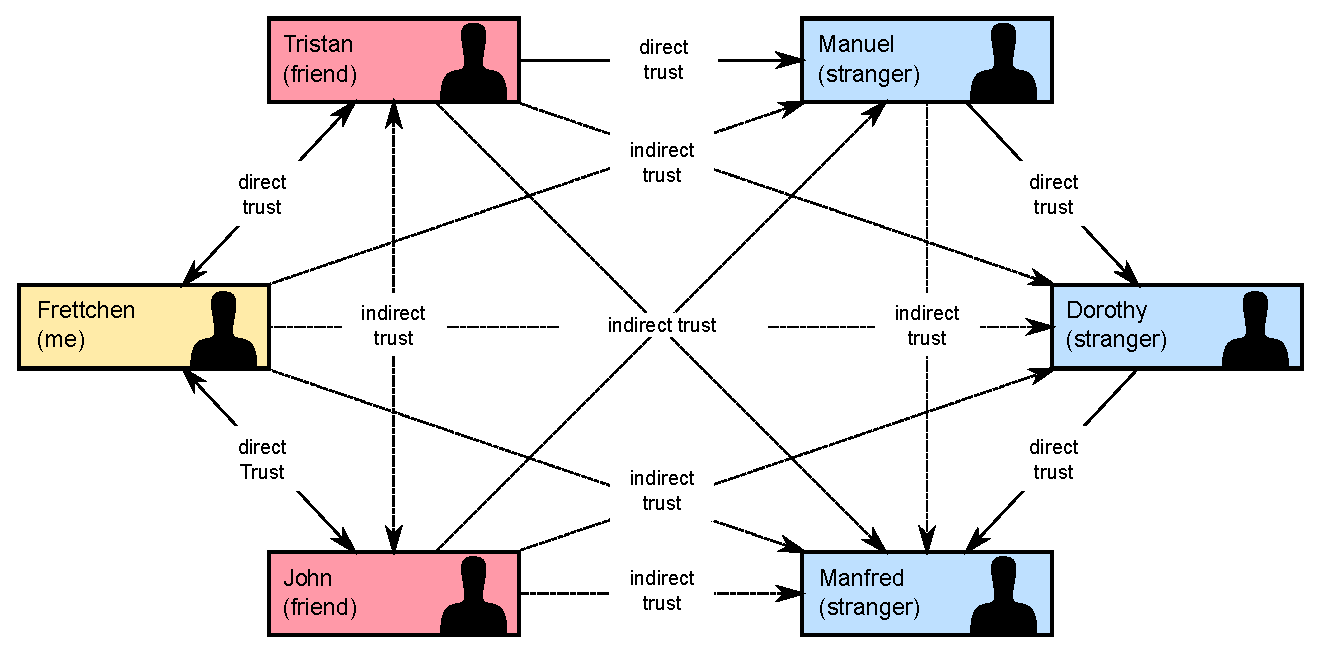
\includegraphics[width=\linewidth]{images/Web_of_Trust.eps}
\end{slide}

\begin{slide}{Trust model}
  \begin{itemize}
  \item In practice trust is subjective.
  \item For example, Blake's key is valid to Alice since she signed
    it, but she may not trust Blake to properly validate keys that he
    signs.
  \item The web of trust model accounts for this by associating with
    each public key on your keyring an indication of how much you
    trust the key's owner:
    \begin{itemize}
    \item unknown, none, marginal, full, ultimate
    \end{itemize}
  \item A key's trust level is something that you alone assign to the
    key, and it is considered private information.
  \item It is not packaged with the key when it is exported; it is
    even stored separately from your keyrings in a separate database.
  \end{itemize}
\end{slide}

\makeatletter\renewcommand{\verbatim@font}{\scriptsize\tt}\makeatother
\begin{slide}[method=direct]{Assigning trust}
\vspace{-10mm}
\begin{verbatim}
$ gpg --edit-key John
...

pub  2048R/65B46947  created: 2016-08-15  expires: never       usage: SC  
                     trust: unknown       validity: full
sub  2048R/4D993DDE  created: 2016-08-15  expires: never       usage: E   
[  full  ] (1). John Smith <smith@example.com>

gpg> trust
pub  2048R/65B46947  created: 2016-08-15  expires: never       usage: SC  
                     trust: unknown       validity: full
sub  2048R/4D993DDE  created: 2016-08-15  expires: never       usage: E   
[  full  ] (1). John Smith <smith@example.com>

Please decide how far you trust this user to correctly verify other users' keys
(by looking at passports, checking fingerprints from different sources, etc.)

  1 = I don't know or won't say
  2 = I do NOT trust
  3 = I trust marginally
  4 = I trust fully
  5 = I trust ultimately
  m = back to the main menu

Your decision?
\end{verbatim}
\end{slide}

\begin{slide}{Using trust to validate keys}
  \begin{itemize}
  \item Formerly, a key was considered valid only if you signed it
    personally (after verifying it).
  \item Now we have a revised model.  A key $K$ is considered valid if
    it meets two conditions:
    \begin{enumerate}
    \item It is signed by enough valid keys, meaning
      \begin{itemize}
      \item you have signed it personally, or
      \item it has been signed by one fully trusted key, or
      \item it has been signed by three marginally trusted keys; and
      \end{itemize}
    \item the path of signed keys leading from $K$ back to your own
      key is five steps or shorter.
    \end{enumerate}
  \end{itemize}
\end{slide}

\begin{slide}[toc=]{}
\centering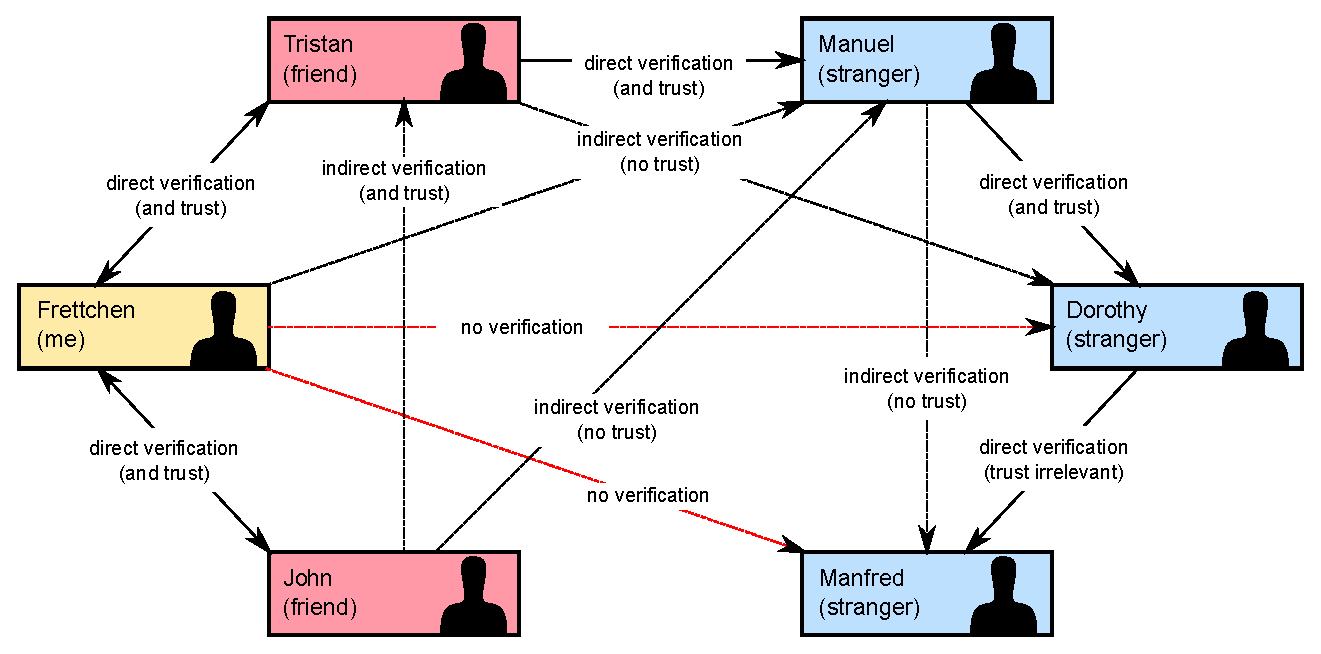
\includegraphics[width=\linewidth]{images/Web_of_Trust_2.eps}
\end{slide}

%=============================================================================
\section{Further topics}
%=============================================================================

\begin{slide}{Conveniences}
  \begin{itemize}
  \item You can use a local configuration file
    (\texttt{\textasciitilde /.gnupg/gpg.conf}) to set your default
    key, preferred key server, \etc
  \item You can use \texttt{gpg-agent}, a daemon that securely caches
    your keys in memory. This way you don't need to type your
    passphrase every time you want to use your key.
  \item \texttt{pinentry} is a collection of programs that will prompt
    for your passphrase using your desktop environment's standard
    dialogs rather than on the terminal.
  \end{itemize}
\end{slide}

\begin{slide}{GUIs}
  There are also a number of full-fledged key management tools which
  let you generate, list, edit, import, export, sign, and publish the
  keys on your keyring.
  \begin{figure}[H]
    \centering
    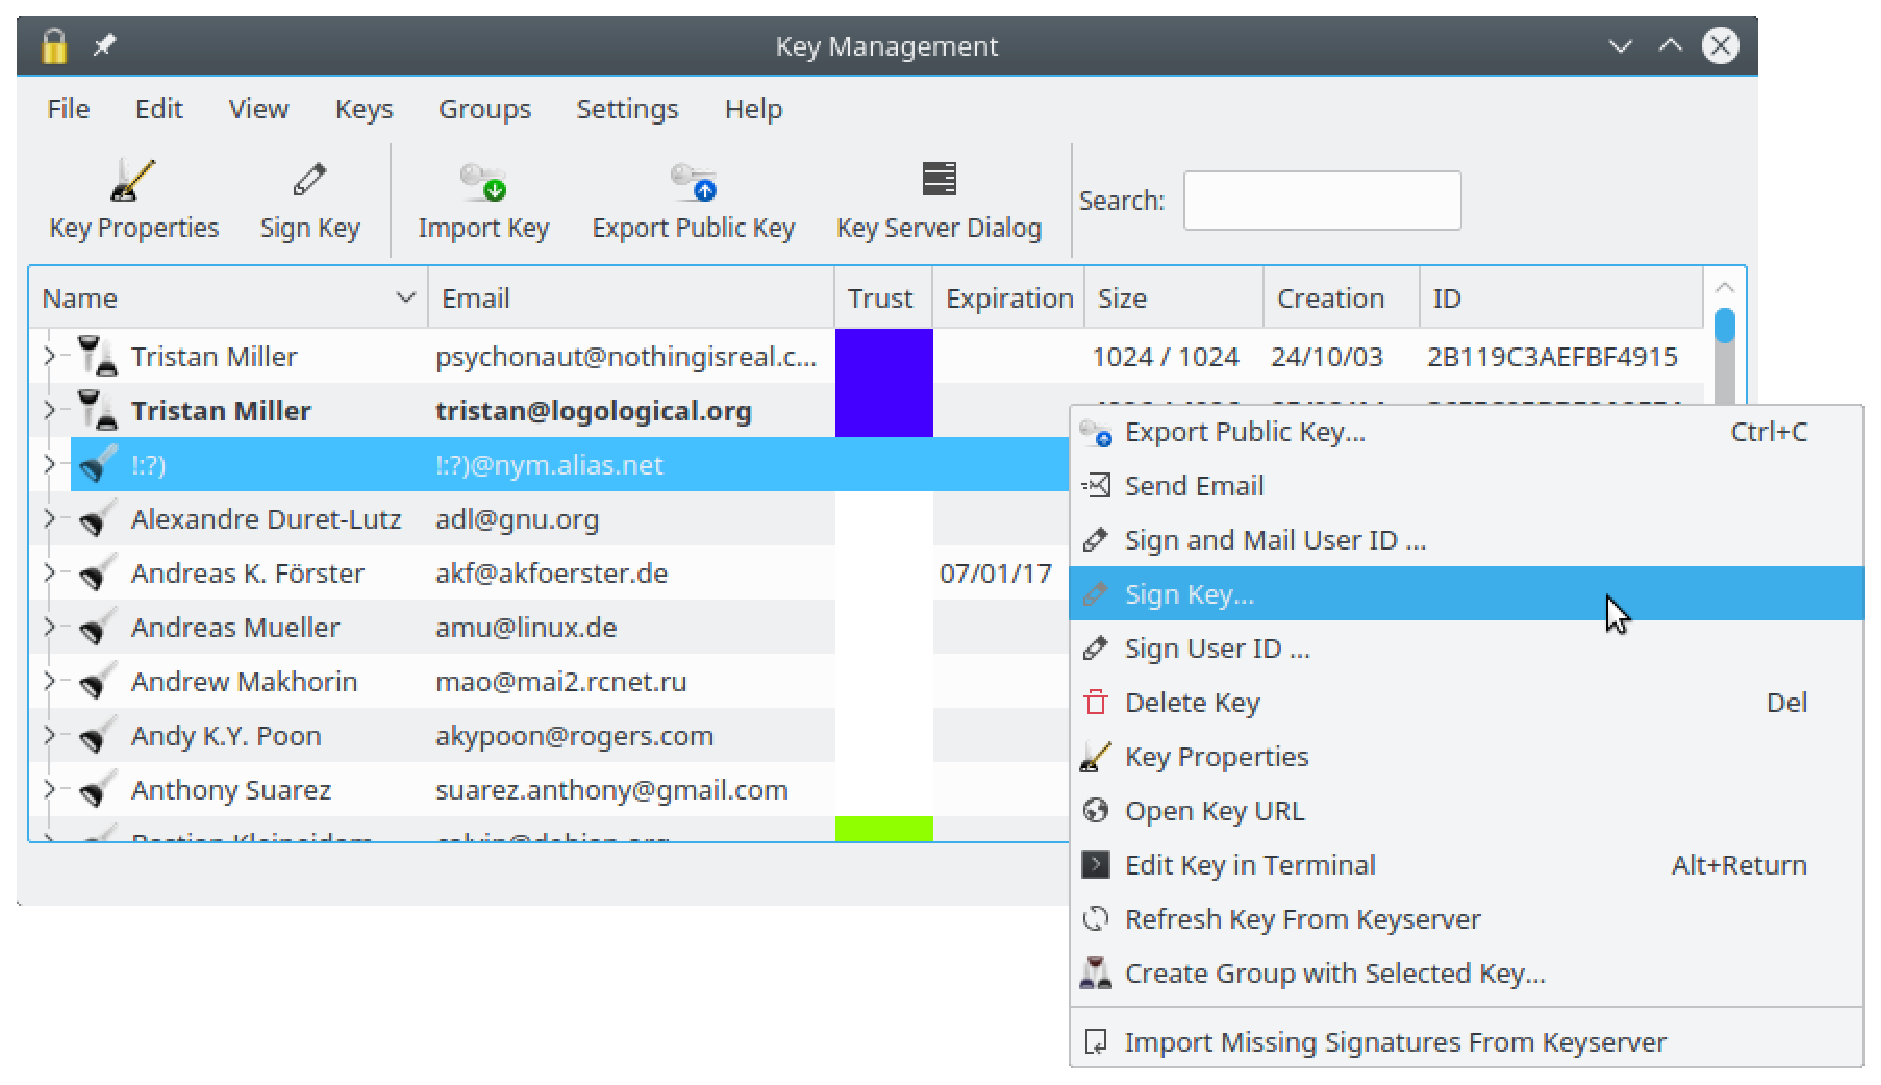
\includegraphics[width=0.75\textwidth]{images/kgpg1.eps}
    \label{fig:kgpg1}
  \end{figure}
\end{slide}

\begin{slide}{E-mail integration}
  Many e-mail clients support GnuPG, natively or via plugins.  For
  each e-mail account or identity, you can associate a public key for
  signing and encryption.
  \begin{figure}[H]
    \centering
    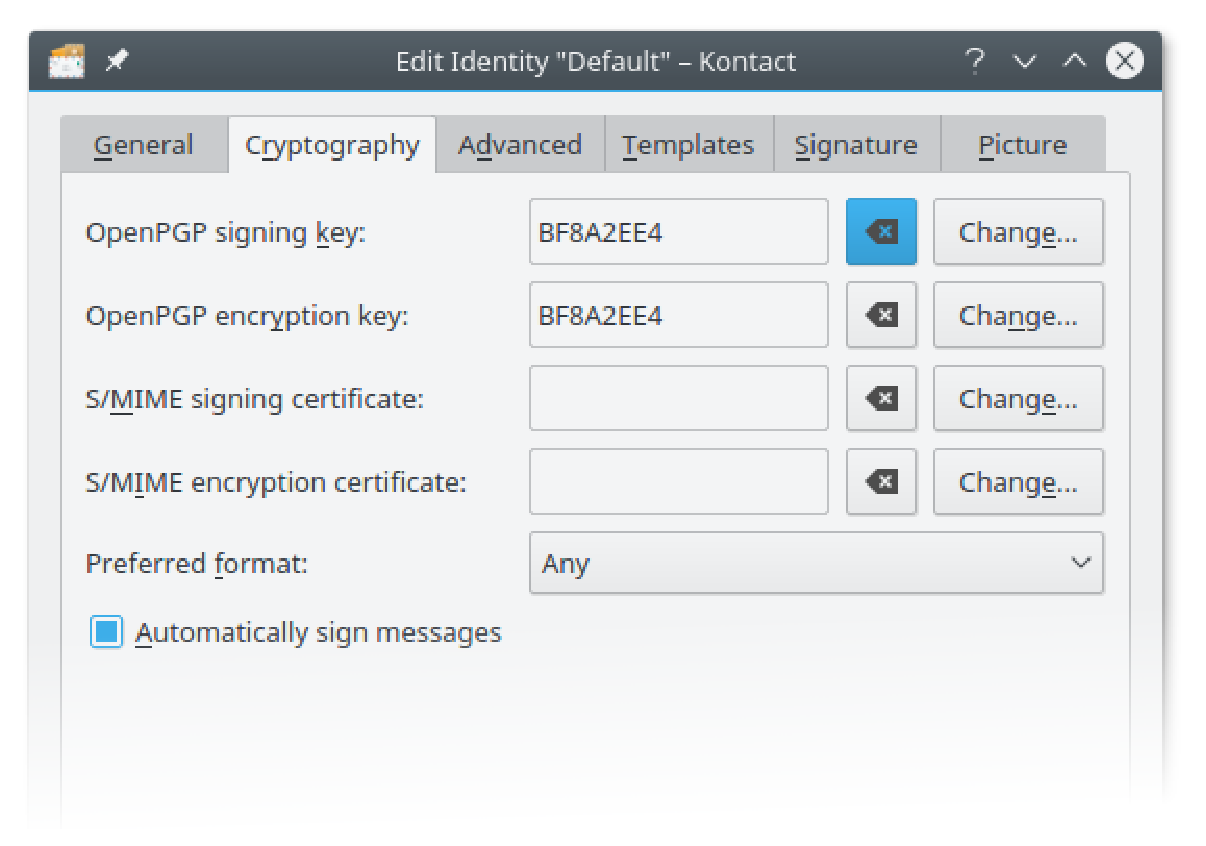
\includegraphics[width=0.6\textwidth]{images/kmail_conf.eps}
    \label{fig:kmail_conf}
  \end{figure}
\end{slide}

\begin{slide}[toc=]{E-mail integration}
  Signatures on messages are automatically checked.
  \begin{figure}[H]
    \centering
    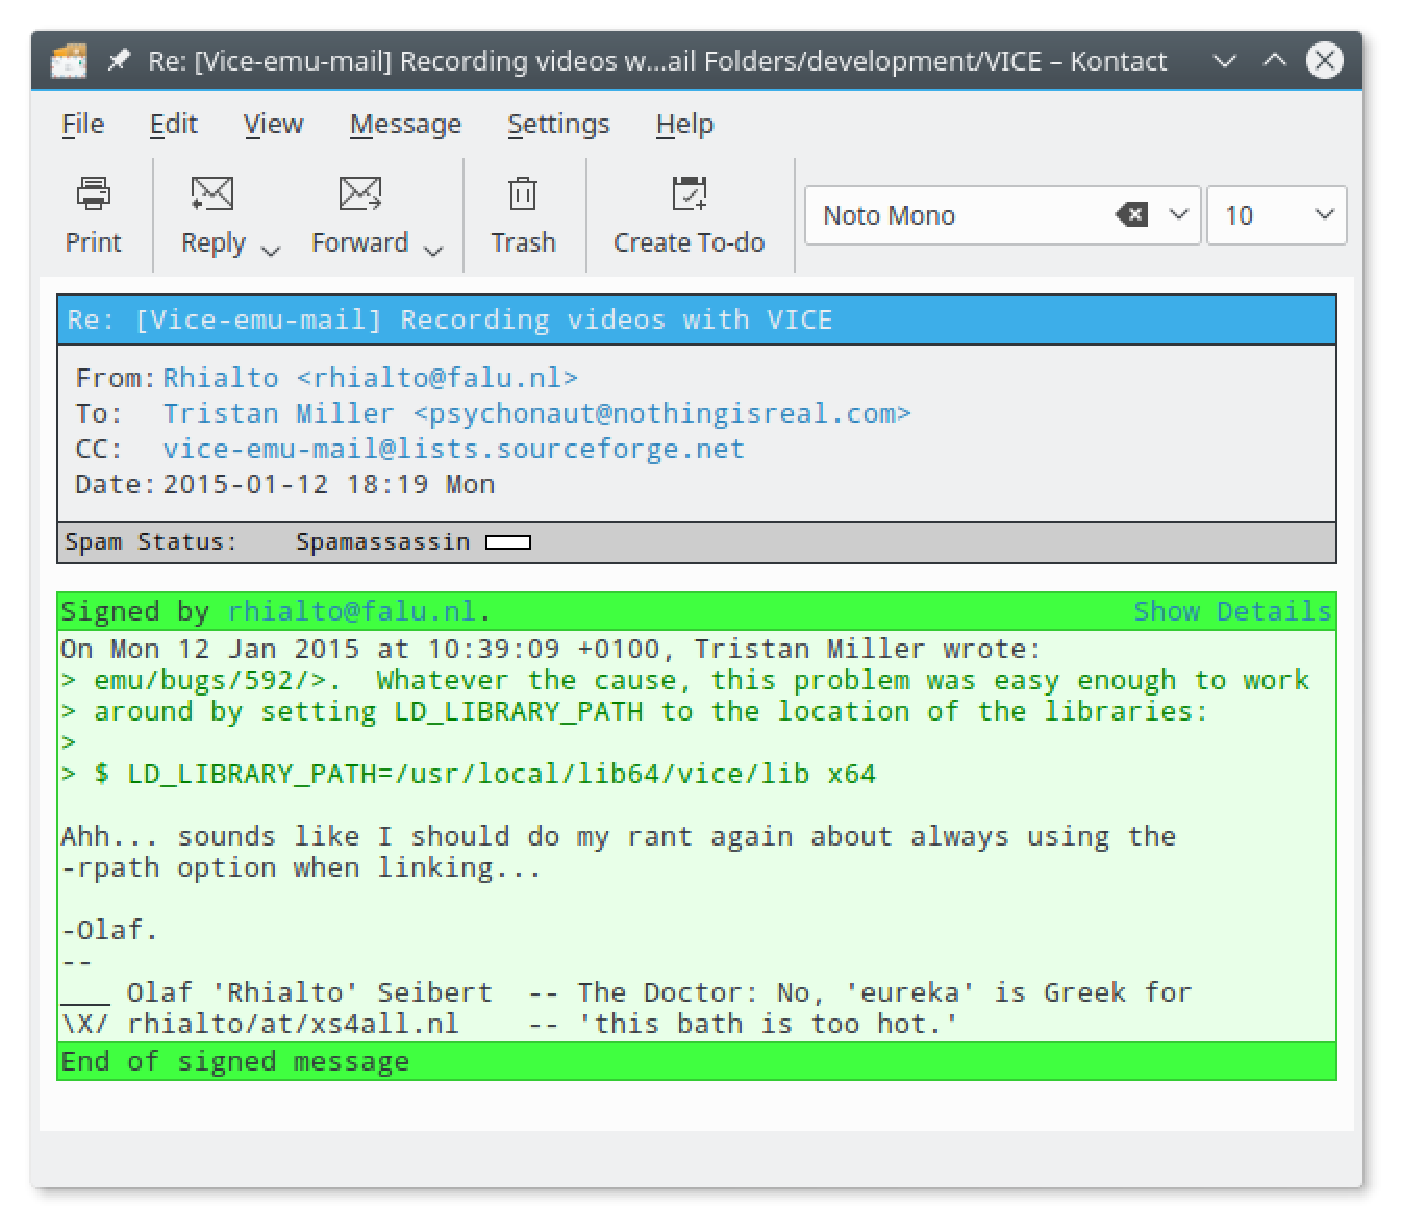
\includegraphics[width=0.6\textwidth]{images/kmail_recvd.eps}
    \label{fig:kmail_recvd}
  \end{figure}
\end{slide}

\begin{slide}[toc=]{E-mail integration}
  In the message composer, you are given the choice of signing and/or
  encrypting the message.
  \begin{figure}[H]
    \centering
    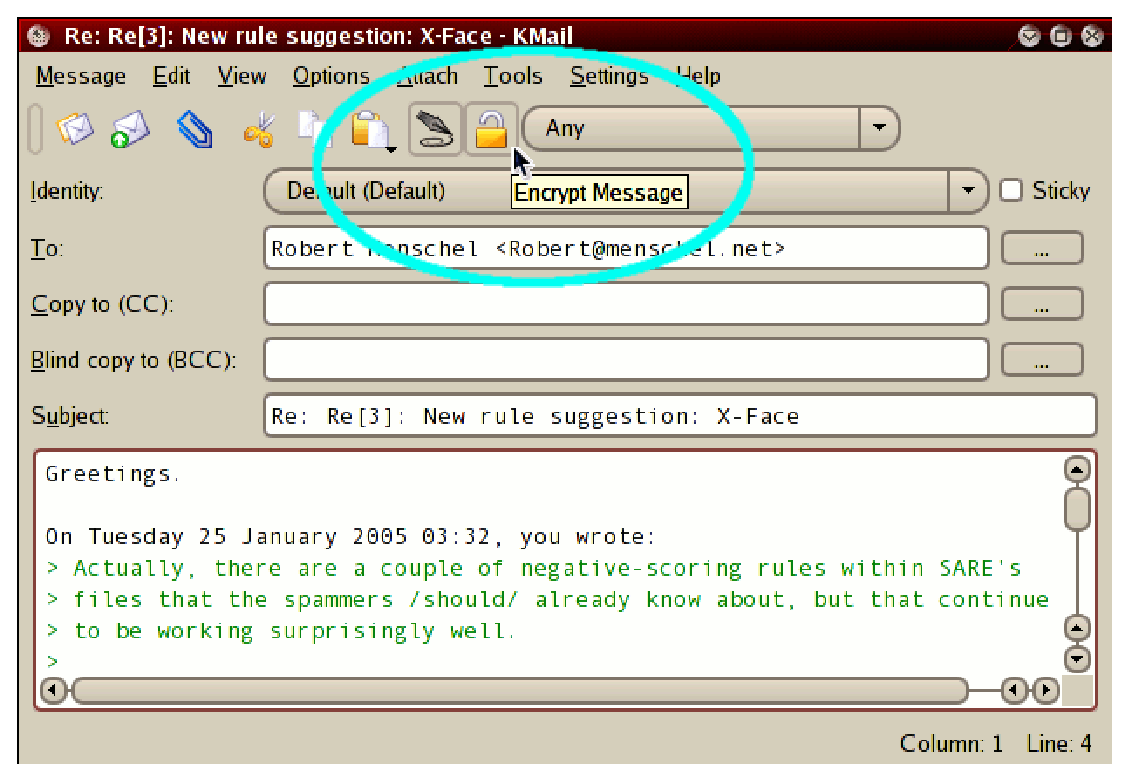
\includegraphics[width=0.7\textwidth]{images/kmail_send.eps}
    \label{fig:kmail_send}
  \end{figure}
\end{slide}

\makeatletter\renewcommand{\verbatim@font}{\footnotesize\tt}\makeatother
\begin{slide}[method=direct]{Git integration}
  \begin{itemize}
  \item Signing contributions protects your reputation from impostors.
  \item Verifying signed commits before pulling or merging can help
    protect your repository's integrity against impostors.
  \end{itemize}

Setting a default signing key:

\vsp
\begin{verbatim}
$ git config --global user.signingkey 4116CBB0
\end{verbatim}

Signing and verifying tags:

\vsp
\begin{verbatim}
$ git tag -s v1.5 -m 'my signed 1.5 tag'
$ git tag -v v1.5
\end{verbatim}

Signing and verifying commits:

\vsp
\begin{verbatim}
$ git commit -S -m 'signed commit'
$ git log --show-signature
$ git merge --verify-signatures signed-branch
\end{verbatim}
\end{slide}

\begin{slide}{Packaging integration}
  \begin{itemize}
  \item Many software packaging and release tools support GnuPG,
    natively or via plugins.
  \item The Maven release plugin handles this automatically (at least
    for binary releases).
  \item For manually posting source or binary releases on the Web or
    on GitHub, produce a detached signature of the release and upload
    it alongside the release.
  \end{itemize}
\end{slide}

\begin{slide}{Identity management}
  \begin{itemize}
  \item Your keypair can include several user IDs (name, e-mail, and
    comment) for each of your identities
    \begin{itemize}
    \item Advantages: convenient (only one keypair to worry about)
    \item Disadvantage: all your identities are publically linked to
      each other
    \end{itemize}
  \item If you have an identity you want to keep separate, then you
    must generate a separate keypair for it.
  \end{itemize}
\end{slide}

\begin{slide}{Key-signing parties}
  \begin{itemize}
  \item A key-signing party is an event at which people present their
    public keys fingerprints to each other, so that they can later
    sign the keys and extend the web of trust:
    \begin{itemize}
    \item Before the party, participants send their key fingerprints
      to the organizer, who prepares a master list.
    \item At the party, the organizer posts the master list and
      distributes a printed copy to each participant.
    \item Each participant declares whether their identity and
      fingerprint on the lists is correct.
    \item Each participant then verifies the identity of every other
      participant, and marks the entry on the list.
    \item After the party, participants sign the keys that passed the
      identity check, and then upload them to the key server.
    \end{itemize}
  \end{itemize}
\end{slide}

\begin{slide}{Online resources}
  \begin{itemize}
  \item \href{https://gnupg.org/}{GnuPG home page} and \href{https://www.gnupg.org/faq/gnupg-faq.html}{FAQ}
  \item \href{http://security.stackexchange.com/questions/tagged/gnupg}{InfoSec Stack Exchange questions on GnuPG}
  \item \href{https://riseup.net/en/security/message-security/openpgp/best-practices}{OpenPGP Best Practices} from Riseup
  \item \href{https://keybase.io/}{Keybase}
  \item \href{http://www.openpgp-courses.org/}{OpenPGP courses and lobbying}
  \item \href{http://cryptnet.net/fdp/crypto/keysigning_party/en/keysigning_party.html}{The Keysigning Party HOWTO}
  \item
    \href{https://wiki.debian.org/Creating\%20signed\%20GitHub\%20releases}{Creating
      signed GitHub releases}
  \item \href{https://mikegerwitz.com/papers/git-horror-story}{A Git
      Horror Story: Repository Integrity with Signed Commits}
  \end{itemize}
\end{slide}

\begin{slide}[toc=]{}
\centering

\vfill

{\huge \textbf{Thank you!}}

\vfill

\tiny Image credits:
\href{https://commons.wikimedia.org/wiki/File:Web_of_Trust.svg}{Web of
  Trust} \copyright\,2009 Ogmios. CC-BY-SA~3.0.
\href{https://commons.wikimedia.org/wiki/Category:Orange_blue_cryptography_diagrams}{Orange
  blue cryptography diagrams} by Bananenfalter. CC0~1.0.
\end{slide}

\end{document}

%%% Local Variables: 
%%% mode: latex
%%% TeX-PDF-mode: t
%%% TeX-PDF-via-dvips-ps2pdf: t
%%% TeX-master: t
%%% End: 
